\documentclass[11pt]{article}

\usepackage[margin=1in]{geometry}
\usepackage{amsmath,amssymb}
\usepackage{booktabs}
\usepackage{graphicx}
\usepackage{tabularx}
\usepackage{microtype}

\title{Result 2.\\
Hydrodynamic entropy of GraphCast:\\
spherical-harmonic power of the latent field}
\author{}
\date{}

\begin{document}
\maketitle

\section{What is being measured}

Result 1 assigns an energy to each mesh length by applying the mesh-edge encoder to the edges of that length. This result assigns the energy differently. GraphCast Small is run for one forecast step, and the latent vector on each mesh node is kept after the encoder and after every processor step. That field is expanded in spherical harmonics. \(E(\ell)\) is the power at degree \(\ell\).

The same entropy is then computed from those powers, grouped into the six mesh levels of this checkpoint:
\[
p_i = \frac{E_i}{\sum_j E_j},
\qquad
H = -\sum_i p_i \ln p_i,
\qquad
H_n = \frac{H}{\ln N}.
\]
\(H\) is in nats. Six bands give \(\ln 6 = 1.792\). The wavenumber of band \(m\) is \(k = 1/L(m)\), with the same lengths as in Result 1,
\[
L(m) = \frac{\pi R}{2 \cdot 2^{m}}, \qquad R = 6371\,\mathrm{km},
\]
from \(10008\,\mathrm{km}\) at \(M_0\) to \(313\,\mathrm{km}\) at \(M_5\). Shorter lengths are absent from this checkpoint and are left out.

\section{Procedure}

The run uses the published GraphCast Small checkpoint: \(1.0^\circ\), 13 pressure levels, mesh size 5, latent size 512, 16 processor steps. Nothing is retrained. The input is the published ERA5 state for 2022-01-01 at \(1.0^\circ\) with 13 pressure levels, normalized with the checkpoint's own per-level mean and standard deviation. The target is the atmosphere six hours later.

After the grid-to-mesh encoder, and after each of the 16 processor steps, the latent on the mesh nodes is stored. For this mesh that is a matrix of shape \(10242 \times 512\). The decoded 2\,m temperature is kept only as a check that the forecast step ran. Its global mean on this date is \(276.9\,\mathrm{K}\).

Each latent channel is interpolated from the mesh nodes onto the Gauss--Legendre grid whose degree matches the node Nyquist,
\[
\ell_{\max} = \big\lfloor \sqrt{10242} \big\rfloor - 1 = 100,
\]
by inverse-distance weighting from the eight nearest mesh vertices. The channel is expanded in orthonormal spherical harmonics, and the power at degree \(\ell\) is the sum of squared coefficients over order and over the 512 channels. The degree \(\ell = 0\) term is the spatial mean of the latent and is left out of \(H\).

Degrees are grouped into octave bands aligned with the mesh. A spherical harmonic of degree \(\ell\) has wavelength \(2\pi R / \ell\). Setting that equal to \(L(m)\) gives the characteristic degree \(\ell(m) = 2^{m+2}\). Band \(M_m\) runs from \(\ell(m-1)+1\) through \(\ell(m)\), with the first band starting at \(\ell = 1\):

\begin{center}
\begin{tabular}{lcccccc}
\toprule
& \(M_0\) & \(M_1\) & \(M_2\) & \(M_3\) & \(M_4\) & \(M_5\) \\
\midrule
degrees & 1--4 & 5--8 & 9--16 & 17--32 & 33--64 & 65--100 \\
\bottomrule
\end{tabular}
\end{center}

The characteristic degree of \(M_5\) is 128, which lies above the node Nyquist, so that band stops at \(\ell = 100\). The energy of a band is the sum of \(E(\ell)\) inside it. The slope quoted as ``band'' is the fit of that band energy against \(k = 1/L(m)\). The slope quoted as ``degree'' is the fit of \(E(\ell)\) itself for \(\ell \ge 2\).

\section{Results}

\(H\) rises at every processor step, and the share of band energy on \(M_0\) falls at every step.

\begin{center}
\begin{tabular}{lrrrr}
\toprule
Step & \(H\) (nats) & \(H_n\) & band slope & share on \(M_0\) \\
\midrule
Encoder & 1.218 & 0.680 & \(-1.525\) & 55.0\% \\
1 & 1.253 & 0.699 & \(-1.462\) & 52.9\% \\
2 & 1.269 & 0.708 & \(-1.423\) & 52.1\% \\
3 & 1.283 & 0.716 & \(-1.380\) & 51.6\% \\
4 & 1.295 & 0.723 & \(-1.355\) & 51.1\% \\
5 & 1.303 & 0.727 & \(-1.333\) & 50.8\% \\
6 & 1.312 & 0.733 & \(-1.316\) & 50.3\% \\
7 & 1.322 & 0.738 & \(-1.297\) & 49.7\% \\
8 & 1.331 & 0.743 & \(-1.296\) & 48.9\% \\
9 & 1.338 & 0.747 & \(-1.286\) & 48.5\% \\
10 & 1.347 & 0.752 & \(-1.262\) & 47.9\% \\
11 & 1.354 & 0.756 & \(-1.264\) & 47.3\% \\
12 & 1.360 & 0.759 & \(-1.249\) & 47.0\% \\
13 & 1.381 & 0.771 & \(-1.232\) & 45.2\% \\
14 & 1.394 & 0.778 & \(-1.203\) & 44.5\% \\
15 & 1.442 & 0.805 & \(-1.146\) & 39.7\% \\
16 & 1.519 & 0.848 & \(-1.015\) & 28.5\% \\
\bottomrule
\end{tabular}
\end{center}

The coefficient of determination of the band fit is \(0.90\) at the encoder, \(0.87\) at step 8, and \(0.76\) at step 16. By the last step the six probabilities are \(0.285\), \(0.251\), \(0.261\), \(0.146\), \(0.051\), \(0.006\). From \(M_0\) to \(M_2\) the band energies are then close, and the decay sits in \(M_3\)--\(M_5\). Inside the bands the per-degree spectrum is steeper: \(E(\ell) \propto \ell^{-2.35}\) at step 16, with coefficient of determination \(0.91\). At the encoder that per-degree slope is \(-2.78\).

\begin{figure}[ht]
\centering
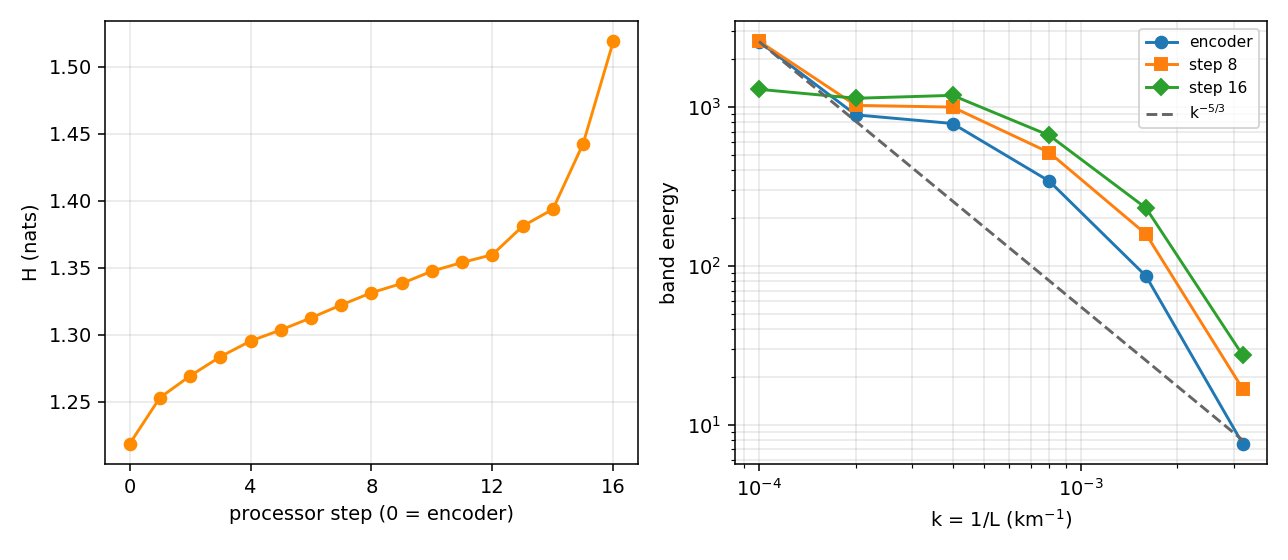
\includegraphics[width=\textwidth]{outputs/graphcast_latent_spectrum.png}
\caption{Left: entropy of the six band energies after the encoder (step 0) and after each processor step. Right: band energy against \(k = 1/L\). The dashed line is \(k^{-5/3}\), drawn through the encoder's \(M_0\) band.}
\end{figure}

\section{Comparison with the local baseline}

The notebooks in \texttt{Main codes} are the baseline, on the same GraphCast Small checkpoint and the same six lengths \(M_0\)--\(M_5\). They use only \texttt{linear\_0} of the mesh-edge encoder, the \(4 \times 512\) matrix. The input of an edge is \((\Delta x, \Delta y, \Delta z, \|\Delta\|)\), and the energy of a level is the mean of \(\|W_0\mathbf{x}+\mathbf{b}_0\|^2\) over the edges of that level. No ERA5 field is loaded, and the second linear map, the layer norm, the 16 processor steps, and the decoder are not evaluated. Those notebooks report the entropy in bits. The row below converts that number to nats: \(1.205\) bits is \(0.835\) nats. \(H_n = 0.466\) is unchanged by the change of base.

\noindent
\begin{tabularx}{\textwidth}{@{}lXX@{}}
\toprule
& Local notebooks & This calculation \\
\midrule
Checkpoint
  & GraphCast Small, published weights
  & The same checkpoint \\
Input
  & Four geometric numbers on each mesh edge
  & Normalized ERA5 state for 2022-01-01 \\
Depth
  & First matrix of the mesh-edge encoder
  & Encoder output and all 16 processor steps \\
\(E\)
  & Mean squared output of the first matrix
  & Band-summed spherical-harmonic power \\
Lengths
  & \(M_0\)--\(M_5\)
  & The same six lengths \\
\bottomrule
\end{tabularx}

\begin{center}
\begin{tabular}{@{}lrrrr@{}}
\toprule
& \(H\) (nats) & \(H_n\) & slope & share on \(M_0\) \\
\midrule
Local \texttt{linear\_0} & 0.835 & 0.466 & \(-1.866\) & 70.5\% \\
Latent field, encoder & 1.218 & 0.680 & \(-1.525\) & 55.0\% \\
Latent field, step 16 & 1.519 & 0.848 & \(-1.015\) & 28.5\% \\
\bottomrule
\end{tabular}
\end{center}

The local slope is the fit of mean \(\|W_0\mathbf{x}+\mathbf{b}_0\|^2\) against \(k = 1/L\), with coefficient of determination \(0.9995\). The other two slopes are the band fits already quoted above. On the local baseline the six probabilities are \(0.705\), \(0.217\), \(0.058\), \(0.015\), \(0.004\), \(0.001\). After processor step 16 they are \(0.285\), \(0.251\), \(0.261\), \(0.146\), \(0.051\), \(0.006\).

The baseline value \(0.835\) nats is fixed by the mesh. A long edge has a much larger input vector than a short one, and \(\|\mathbf{x}\|^2\) scales as length squared. Length halves at each refinement, so the energy falls by about a factor of four and the slope sits near \(-2\). About \(70\%\) of that energy lies on \(M_0\). The same entropy, to three decimals, appears for the operational and full checkpoints in those notebooks, which is what a shared geometric input produces.

The latent-field entropy uses the same formula on a different energy. At the encoder, \(H = 1.218\) nats and \(H_n = 0.680\), because \(M_0\) holds \(55\%\) rather than \(70\%\) and the middle bands carry a real share. The vector being measured is the latent weather state on the mesh nodes. Edge length does not set its size. The further rise from \(1.218\) to \(1.519\) nats is the processor. Each of the 16 steps mixes that latent across edges of every length, and by the last step \(M_0\), \(M_1\), and \(M_2\) hold comparable power. The local calculation has no depth, so it has no such trajectory.

\end{document}
